\documentclass[11pt,a4paper]{article}

\usepackage[utf8]{inputenc}
\usepackage{amsmath}
\usepackage{amsfonts}
\usepackage{amssymb}
\usepackage{graphicx}
\usepackage{hyperref}
\usepackage{geometry}
\usepackage{booktabs}
\usepackage{caption}
\usepackage{subcaption}
\usepackage{float}
\usepackage{xcolor}

\geometry{margin=1in}

% Status callouts. Deliberately built from xcolor alone -- no tcolorbox, mdframed or
% other extra package -- so this file compiles with a base LaTeX installation.
% Both environments break across pages.
\definecolor{gapred}{rgb}{0.62,0.13,0.10}
\definecolor{okgreen}{rgb}{0.09,0.38,0.20}

\newenvironment{gapbox}[1]{%
  \par\medskip\noindent
  \textcolor{gapred}{\rule{\linewidth}{1.1pt}}\par\nobreak\vspace{2pt}%
  \noindent\textcolor{gapred}{\textbf{NOT CURRENTLY REPRODUCED --- #1}}%
  \par\nobreak\vspace{3pt}%
  \begingroup\leftskip=1.2em\relax\small
}{%
  \par\endgroup\vspace{3pt}%
  \noindent\textcolor{gapred}{\rule{\linewidth}{0.5pt}}\par\medskip
}

\newenvironment{okbox}[1]{%
  \par\medskip\noindent
  \textcolor{okgreen}{\rule{\linewidth}{1.1pt}}\par\nobreak\vspace{2pt}%
  \noindent\textcolor{okgreen}{\textbf{VERIFIED --- #1}}%
  \par\nobreak\vspace{3pt}%
  \begingroup\leftskip=1.2em\relax\small
}{%
  \par\endgroup\vspace{3pt}%
  \noindent\textcolor{okgreen}{\rule{\linewidth}{0.5pt}}\par\medskip
}

\title{Thalamocortical Gating Project Documentation \\
\large Methodological and Theoretical Foundations}
\author{Thalamocortical Gating Project}
\date{\today}

\begin{document}

\maketitle

\begin{abstract}
This document is the log of our modelling architecture, experimental protocols and
theoretical foundations. It describes the progression from a phenomenological
proof-of-concept model of pathway-specific gating in the prefrontal cortex (PFC) to a
stochastic emergent mechanistic model, both controlled by the mediodorsal thalamus
(MD), alongside the Brian 2 spiking network that implements the underlying circuit
(Section \ref{sec:three}).
Throughout, we distinguish the \emph{intended} behaviour (the project specification)
from the \emph{verified} behaviour of the current code. Claims that the implementation
does not presently reproduce are marked in red boxes rather than removed, since they
remain the target of the work. Section \ref{sec:verification} collects the current
verification status in one place.
\end{abstract}

\section{Project Overview}
The goal of this project is to model and simulate \textbf{pathway-specific gating} in
the prefrontal cortex (PFC), controlled by the mediodorsal thalamus (MD). By
regulating local inhibitory interneurons (VIP, SOM, PV), the MD thalamus should control
which dendritic branches of PFC pyramidal neurons undergo calcium-based synaptic
plasticity, allowing the brain to learn context-specific pathways without catastrophic
forgetting.

\section{Three Implementations}
\label{sec:three}
An important structural point, easy to miss when reading the figures: this project
contains \textbf{three independent implementations}, not one. They agree on parameter
values by convention, but share no code, and each figure in this document comes from
exactly one of them (Table \ref{tab:models}).

\begin{table}[H]
    \centering
    \small
    \begin{tabular}{@{}llp{6.6cm}@{}}
    \toprule
    \textbf{Model} & \textbf{Files} & \textbf{Role} \\ \midrule
    \textbf{A.} Brian 2 spiking network
      & \texttt{src/v2/}, \texttt{experiments/}
      & The full spiking circuit: multi-compartment pyramidal cell, PV/SOM/VIP LIF
        interneurons, MD as a \texttt{PoissonGroup}, native Brian 2
        Graupner-Brunel synapses. \emph{The only model with connection
        probabilities.} Source of Figure \ref{fig:architecture}. \\ \addlinespace
    \textbf{B.} Phenomenological
      & \texttt{main\_gating\_figures.py}
      & Pure NumPy. Hardcoded dendritic inhibition instead of simulated
        interneurons. Source of Figures 1--4. \\ \addlinespace
    \textbf{C.} Emergent mechanistic
      & \texttt{emergent\_gating\_mechanistic\_model.py}
      & Pure NumPy. Inhibition emerges from noisy interneuron rates driven by
        Poisson MD spike counts. Source of the mechanistic figures. \\ \bottomrule
    \end{tabular}
    \caption{The three implementations. Models B and C do not import \texttt{src/v2/}
    and do not use Brian 2, so the parameters of Section \ref{sec:poisson} apply to
    Model A alone.}
    \label{tab:models}
\end{table}

\section{The MD Thalamus as a Poisson Group}
\label{sec:poisson}
This is a key design decision. In \textbf{Model A}, the mediodorsal thalamus is not a
single value or a static current: it is a \textbf{Poisson spiking group}
(\texttt{n\_md}~$=50$ relay cells), a population whose spikes arrive stochastically at
a specified mean rate. This is biologically appropriate because thalamic relay neurons
fire in a largely Poisson-distributed manner.

The MD group does \textbf{not} connect uniformly to all targets. It projects with
different probabilities and different weights to different interneuron types
(\texttt{src/v2/parameters.py}):
\begin{itemize}
    \item \textbf{MD $\rightarrow$ PV:} $p=0.5$, $g_{\text{AMPA}} = 0.12$ nS.
          Intended as broad, non-selective somatic gain control via PV.
    \item \textbf{MD $\rightarrow$ VIP:} $p=0.3$, $g_{\text{AMPA}} = 0.5$ nS.
          Context-selective disinhibitory gating via VIP.
\end{itemize}

\paragraph{A correction to the original rationale.}
Earlier versions of this document argued that MD ``targets PV broadly but VIP more
selectively'' on the basis of the connection probabilities alone ($0.5$ versus $0.3$).
That argument does not survive the arithmetic. The total drive onto a postsynaptic cell
scales as $p \cdot n_{\text{md}} \cdot g$:
\begin{align}
    \text{PV:}\quad  &0.5 \times 50 \times 0.12\,\text{nS} = 3.0\,\text{nS}, \\
    \text{VIP:}\quad &0.3 \times 50 \times 0.5\,\text{nS}\phantom{2} = 7.5\,\text{nS}.
\end{align}
The conductances differ by a factor of $4.2$ in the opposite direction to the
probabilities, so MD drive onto VIP is in fact $2.5\times$ \emph{stronger} in
aggregate. The selectivity distinction between the two pathways must therefore rest on
the sparser \emph{connectivity} of the VIP projection --- fewer, stronger contacts,
giving a higher-variance and more all-or-none response --- and not on total drive.

\begin{figure}[H]
    \centering
    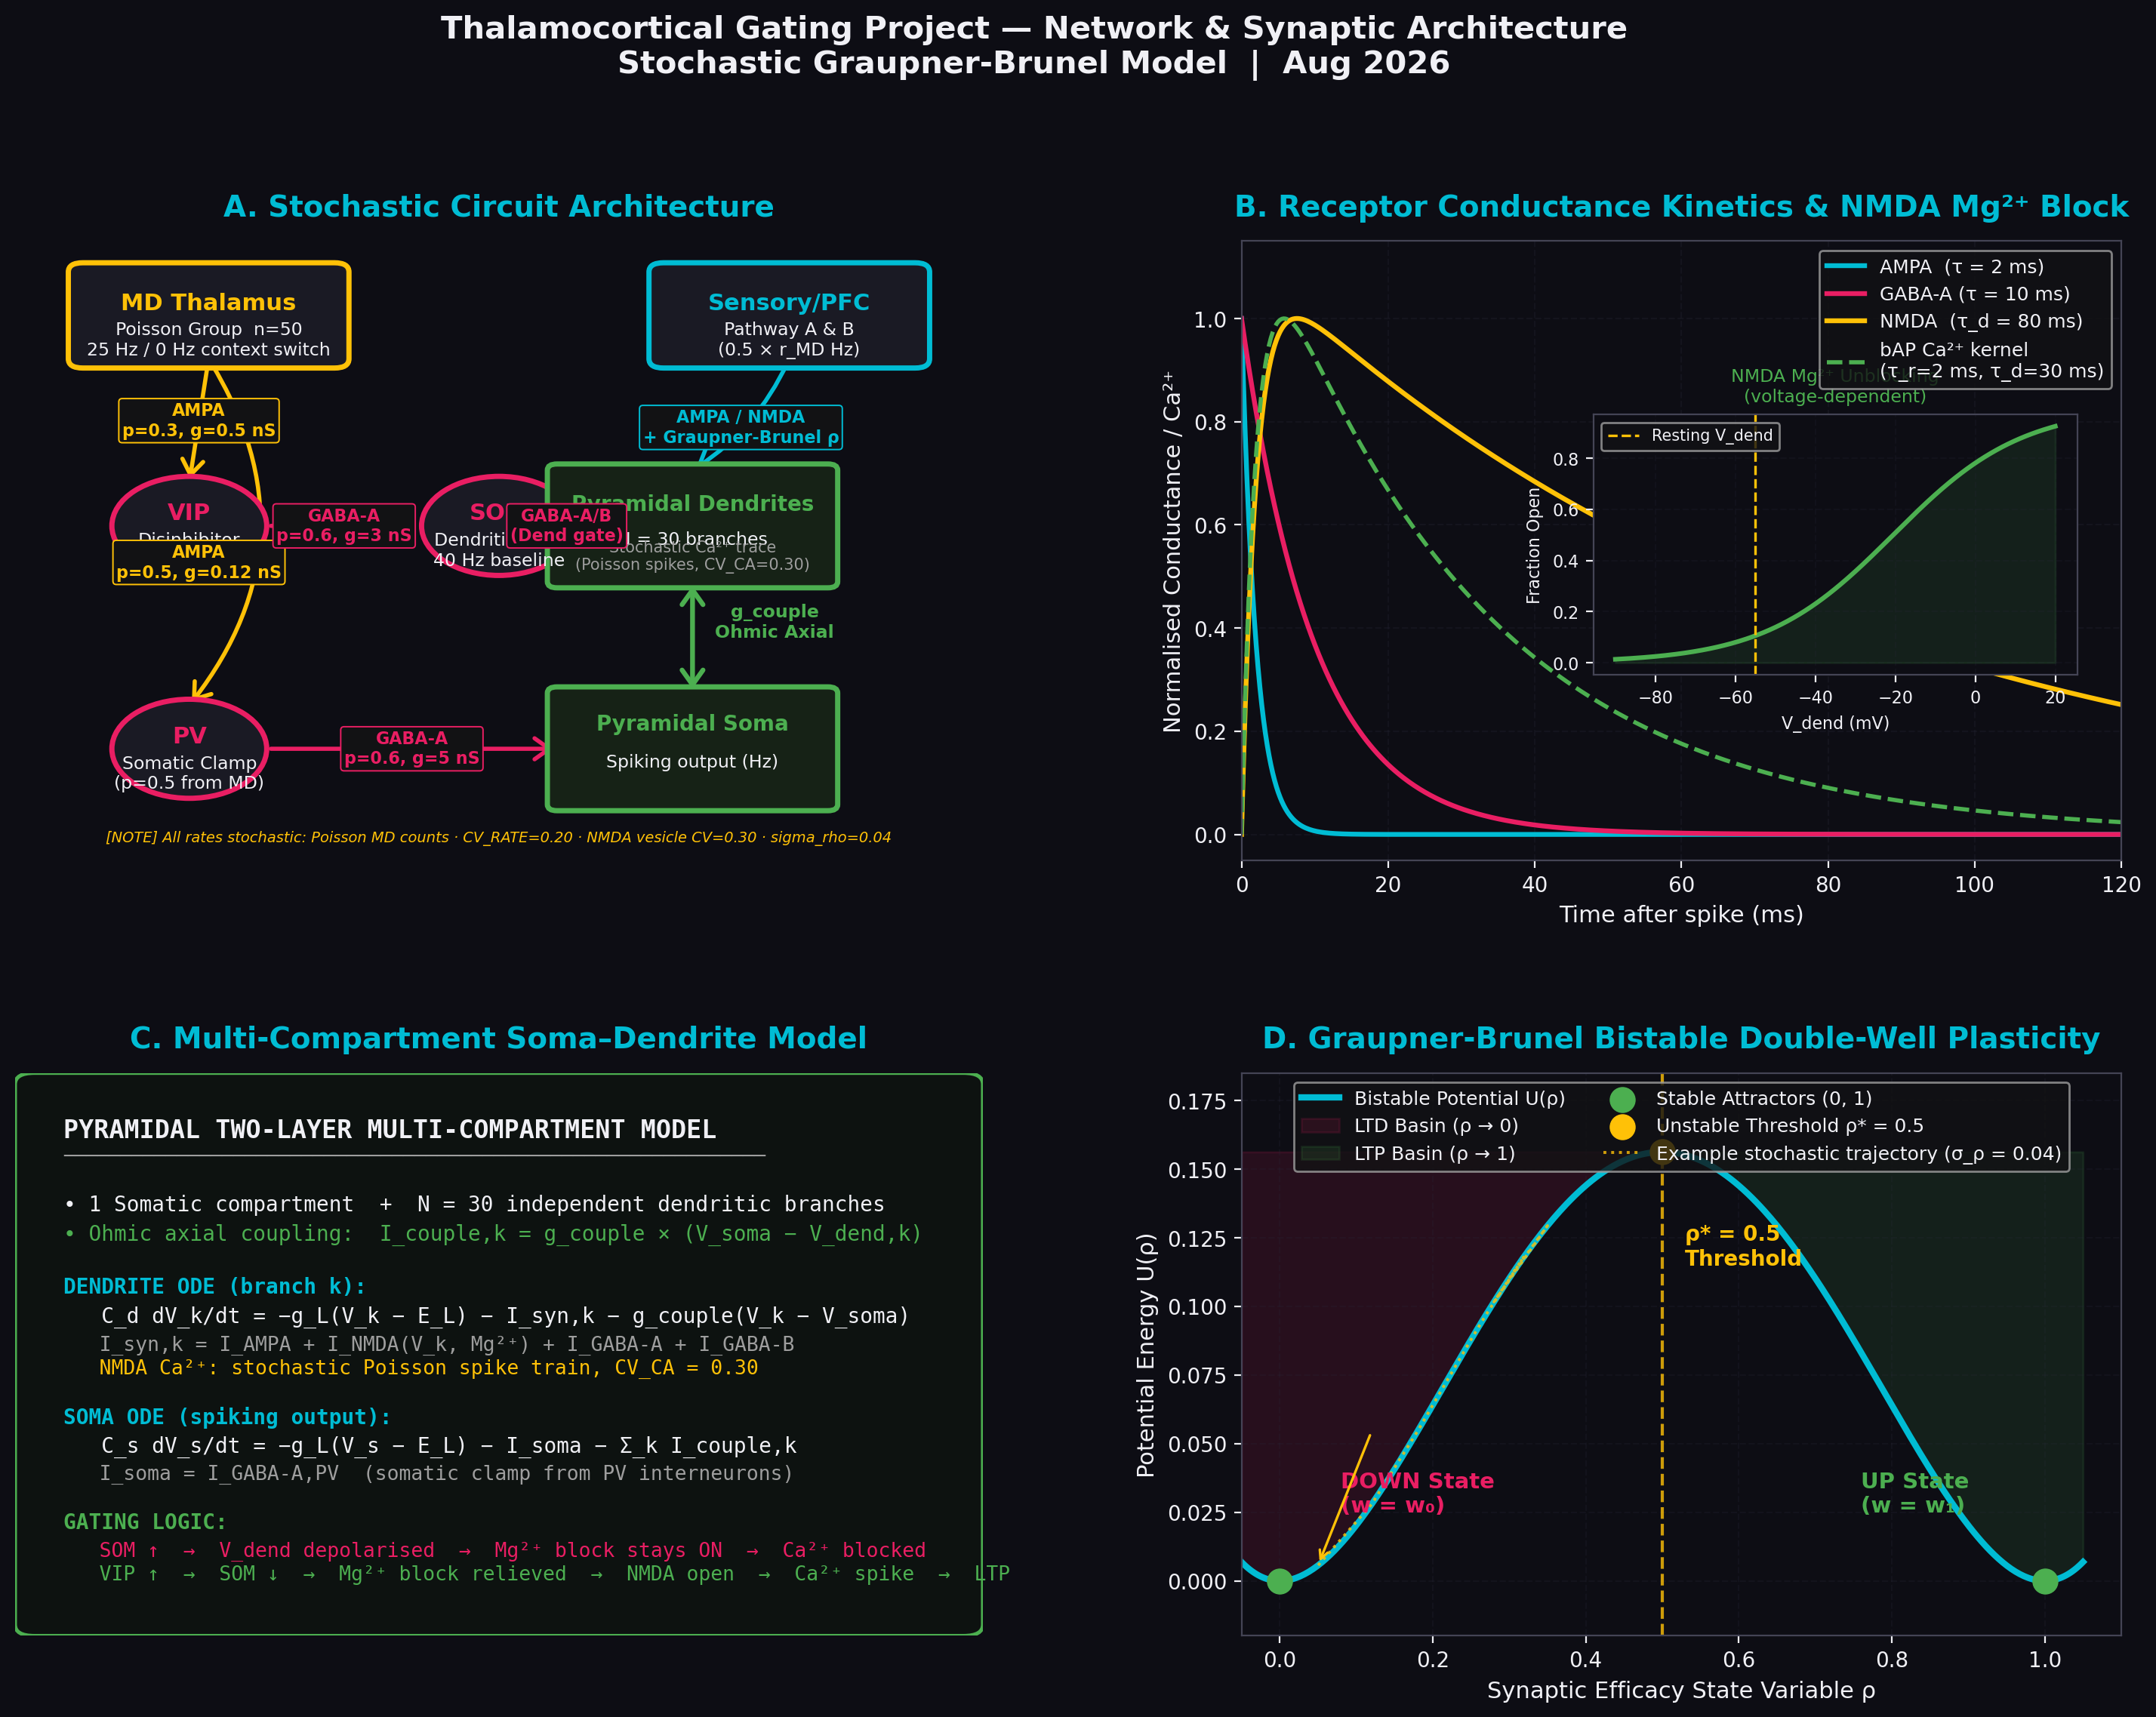
\includegraphics[width=\textwidth]{figures/network_synaptic_architecture.png}
    \caption{Complete network architecture and synaptic wiring, detailing the
    stochastic connections, receptor kinetics and multi-compartmental gating logic.
    Generated by \texttt{experiments/generate\_network\_synapse\_figure.py}.}
    \label{fig:architecture}
\end{figure}

\begin{gapbox}{Figure \ref{fig:architecture} is hand-drawn, not introspected}
\texttt{generate\_network\_synapse\_figure.py} imports no parameters and hardcodes
every annotation, so the diagram can drift from the code. Two labels are currently
wrong: it states $N = 30$ dendritic branches (every runnable script uses \textbf{2}),
and it mixes Model C's parameters (\texttt{CV\_RATE}, $\sigma_\rho$,
$0.5 \times r_{\text{MD}}$) with Model A's ($p$, $g$, $n_{\text{md}}$) as though they
described one model.
\end{gapbox}

\section{Circuit Scale as Implemented (Model A)}
For reference, since these numbers differ from several in-code comments. All values from
\texttt{src/v2/parameters.py} as used by \texttt{experiments/demo\_v2\_zhang2025.py}.

\begin{table}[H]
    \centering
    \small
    \begin{tabular}{@{}lll@{}}
    \toprule
    \textbf{Population} & \textbf{Size} & \textbf{Parameter} \\ \midrule
    Pyramidal soma                & 1           & \texttt{num\_Soma} \\
    Dendritic branches            & \textbf{2}  & \texttt{num\_dend\_each} (per-script override) \\
    MD thalamus (\texttt{PoissonGroup}) & 50    & \texttt{n\_md} \\
    PV interneurons               & 20          & \texttt{n\_pv} \\
    SOM interneurons              & 20          & \texttt{n\_som\_spike} \\
    VIP interneurons              & 20          & \texttt{n\_vip\_spike} \\
    Cortical pathway input        & 30 @ 80 Hz  & literal per script \\ \bottomrule
    \end{tabular}
    \caption{Implemented population sizes. Note the dendrite count: the
    \texttt{parameters.py} default is \texttt{num\_DendEach}~$=10$, but every experiment
    overrides it to 2. The value 30 appears as a branch count only in
    \texttt{src/v2/InterneuronalCircuit.py}, which nothing imports.}
\end{table}

SOM cells receive \textbf{no synaptic excitation}; their baseline rate comes from a
constant bias current \texttt{iBaseline\_som}. Measured: $22$~pA yields
$39.5$~Hz, which is the $\approx 40$~Hz baseline used throughout this document.
Some in-code comments state ``$\sim$10 Hz'' or ``$\sim$30 Hz''; those comments are
incorrect. There is no SOM~$\rightarrow$~PV synapse anywhere in the codebase, despite
\texttt{gGABA\_pv} being defined for one.

\section{The Two Figure-Generating Models}
\textbf{Why two?} We first needed to prove the mathematical theory worked in principle,
and then to test whether the circuit design survives in a messy, biological
environment.

\subsection{A. The Phenomenological Model}
\textit{Proof-of-concept replication of Yang et al. (2016).}

\begin{itemize}
    \item \textbf{Purpose:} To mathematically validate the core theory --- that
      \textit{if} dendritic disinhibition isolates a branch, the Graupner-Brunel
      equations will restrict learning to that branch.
    \item \textbf{Methodology:} It uses \textbf{hardcoded shortcuts} instead of a real
      circuit. Rather than simulating interneurons, the ``disinhibited'' and
      ``inhibited'' branches are assigned fixed inhibition levels directly.
      \emph{Correction:} the code assigns the values $2.0$ and $35.0$ and then scales
      them by \texttt{g\_inh = 0.8 * inh}, so the conductances actually applied are
      \textbf{1.6 nS} and \textbf{28.0 nS} --- not $2.0$ and $35.0$ nS as previously
      stated here. Model C uses a different map
      (\texttt{W\_SOM\_DEND}~$=0.875$ nS/Hz, giving $35$ nS at the $40$ Hz SOM
      baseline), so only Model C reaches $35$ nS.
    \item \textbf{Stochasticity:} This model is \textbf{not deterministic}, as earlier
      drafts of this document claimed. It draws Poisson pathway rates and applies the
      same Gaussian $\rho$ noise and the same accelerated learning rate
      ($\eta_\rho = 0.08$) as Model C. The genuine distinction between the two models
      is \emph{hardcoded versus emergent inhibition}, not deterministic versus
      stochastic.
    \item \textbf{Code \& Figures:} \texttt{main\_gating\_figures.py} ($\approx$3 s),
      writing to \texttt{figures/phenomenological/}.
    \begin{itemize}
        \item \textbf{Figures 1--3} plot continuous-time relations (the STDP curve, the
          static dendritic I/O sigmoid, and the steady-state weight-versus-rate
          relation). Being closed-form rather than time-series, they carry no
          trial-by-trial noise. Note that Figure 3 is a hand-calibrated surrogate
          (\texttt{\_weight\_change\_from\_ca} is, by its own docstring, ``a simplified
          steady-state version''), not the full Graupner-Brunel rule.
        \item \textbf{Figure 4} is a 300-trial simulation of branch-specific learning
          under idealised, hardcoded inhibition.
    \end{itemize}
\end{itemize}

\begin{figure}[H]
    \centering
    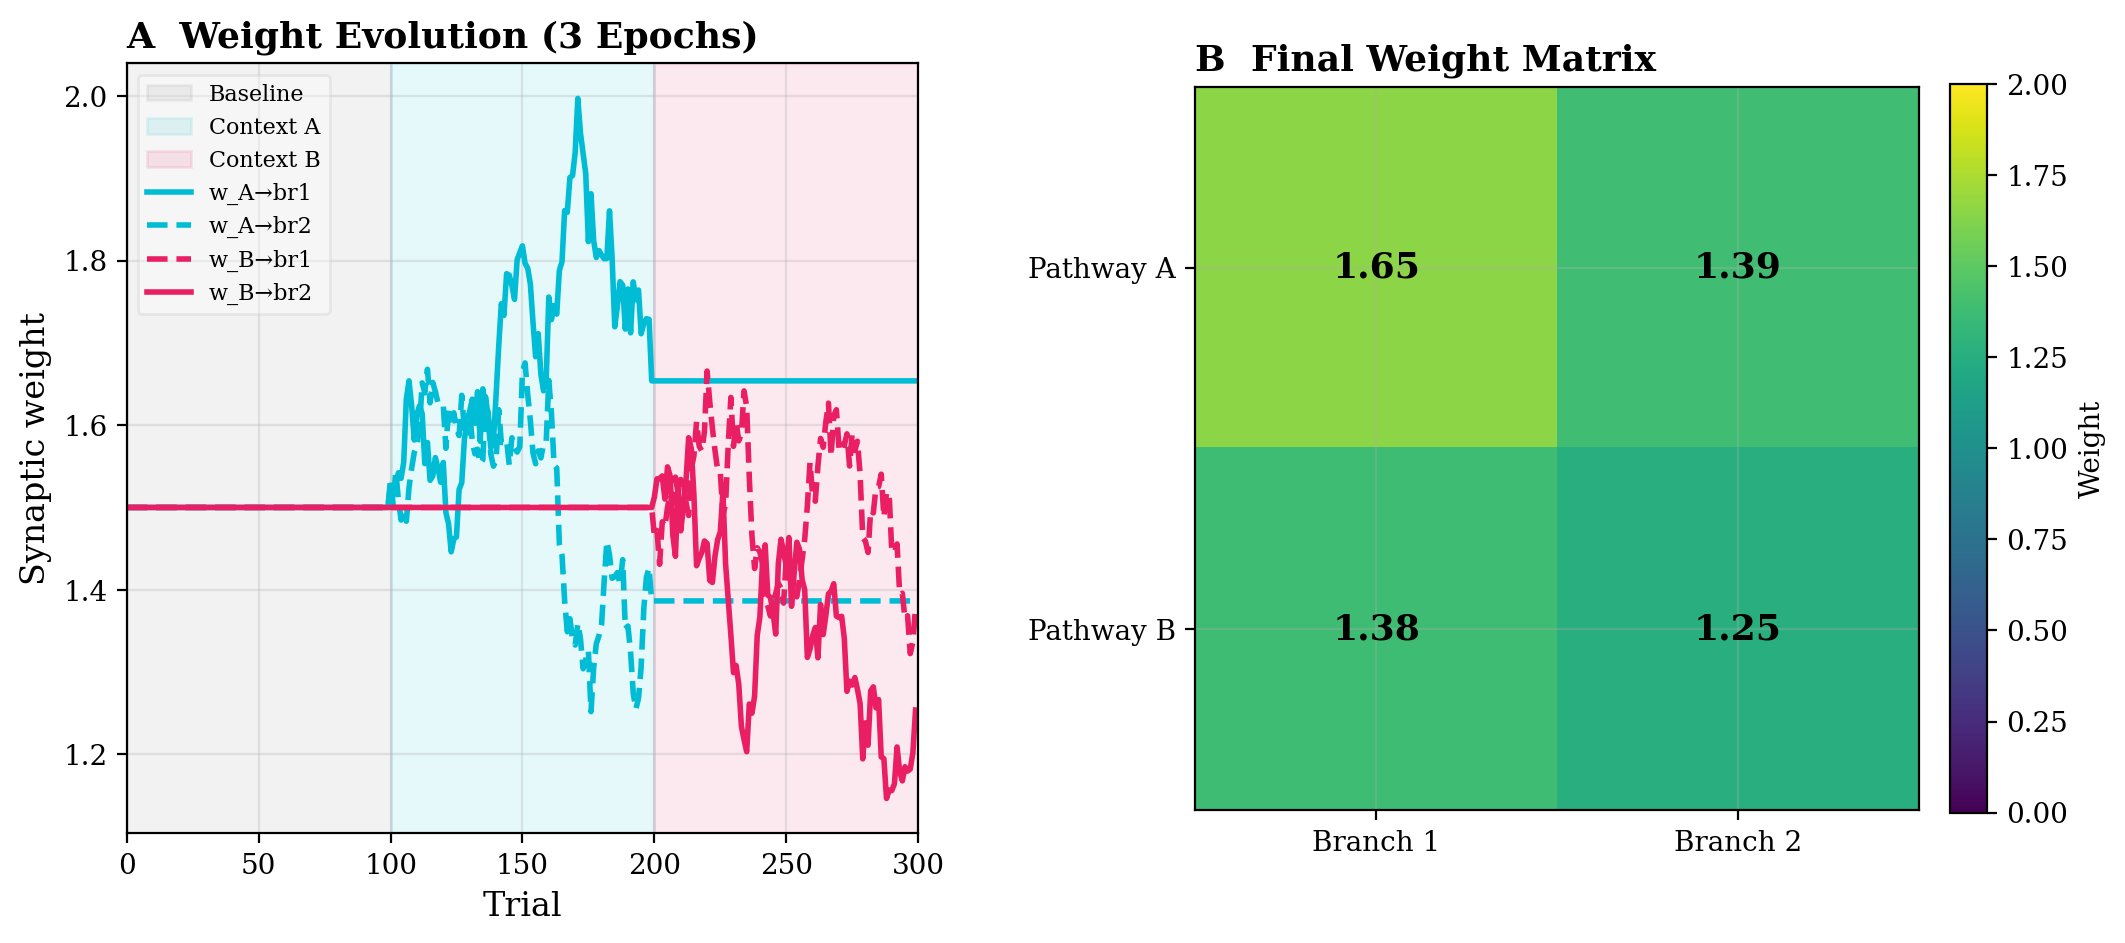
\includegraphics[width=0.85\textwidth]{figures/phenomenological/fig4_branch_specific_learning.png}
    \caption{Phenomenological branch-specific learning using idealised, hardcoded
    inhibition levels (1.6 nS disinhibited, 28.0 nS inhibited).}
    \label{fig:phenom_learning}
\end{figure}

\subsection{B. The Emergent Mechanistic Model}
\textit{Our novel contribution --- fully stochastic.}

\begin{itemize}
    \item \textbf{Purpose:} To test the robustness of the gating mechanism against
      severe biological stochasticity --- whether gating still functions when
      inhibition is not hardcoded but emerges dynamically from noisy interneurons
      driven by erratic Poisson spike trains.
    \item \textbf{Methodology:} Replaces the hardcoded shortcuts with a dynamic
      rate-based circuit (VIP suppresses SOM, SOM inhibits the dendrite):
      $r_{\text{SOM}} = \max(0,\, 40 - 1.5\,r_{\text{VIP}})$ Hz, and the branch
      conductance is $0.875\ \text{nS/Hz} \times r_{\text{SOM}}$. Noise sources:
        \begin{enumerate}
            \item \textbf{Poisson drive:} MD context is a genuine Poisson spike count
              per trial, $n_{\text{spikes}} \sim \text{Poisson}(\lambda T)$.
            \item \textbf{Interneuron variability:} rates carry Gaussian noise with
              \texttt{CV\_RATE}~$=0.20$. \emph{Correction:} this is applied as
              $\sigma = 0.20\,r$, i.e.\ \emph{linear} in the rate. The Fano factor
              therefore grows in proportion to rate rather than remaining $\approx 1$;
              the square-root scaling described in the module docstring is not what the
              code does.
            \item \textbf{Vesicle noise:} NMDA calcium amplitude varies per spike,
              \texttt{CV\_CA}~$=0.30$.
            \item \textbf{Bistable drift:} the $\rho$ update carries Gaussian noise
              ($\sigma_\rho = 0.04$). To make movement visible within 300 trials, an
              accelerated effective learning rate $\eta_\rho = 0.08$ is applied in
              place of the canonical $\tau_\rho = 346.36$ s relaxation, which would
              need $\approx 692$ trials.
        \end{enumerate}
    \item \textbf{Code \& Figures:} \texttt{emergent\_gating\_mechanistic\_model.py}
      ($\approx$4 s), writing to \texttt{figures/mechanistic/}. Seeded with
      \texttt{default\_rng(42)}, so output is reproducible.
\end{itemize}

\begin{figure}[H]
    \centering
    \begin{subfigure}[b]{0.48\textwidth}
        \centering
        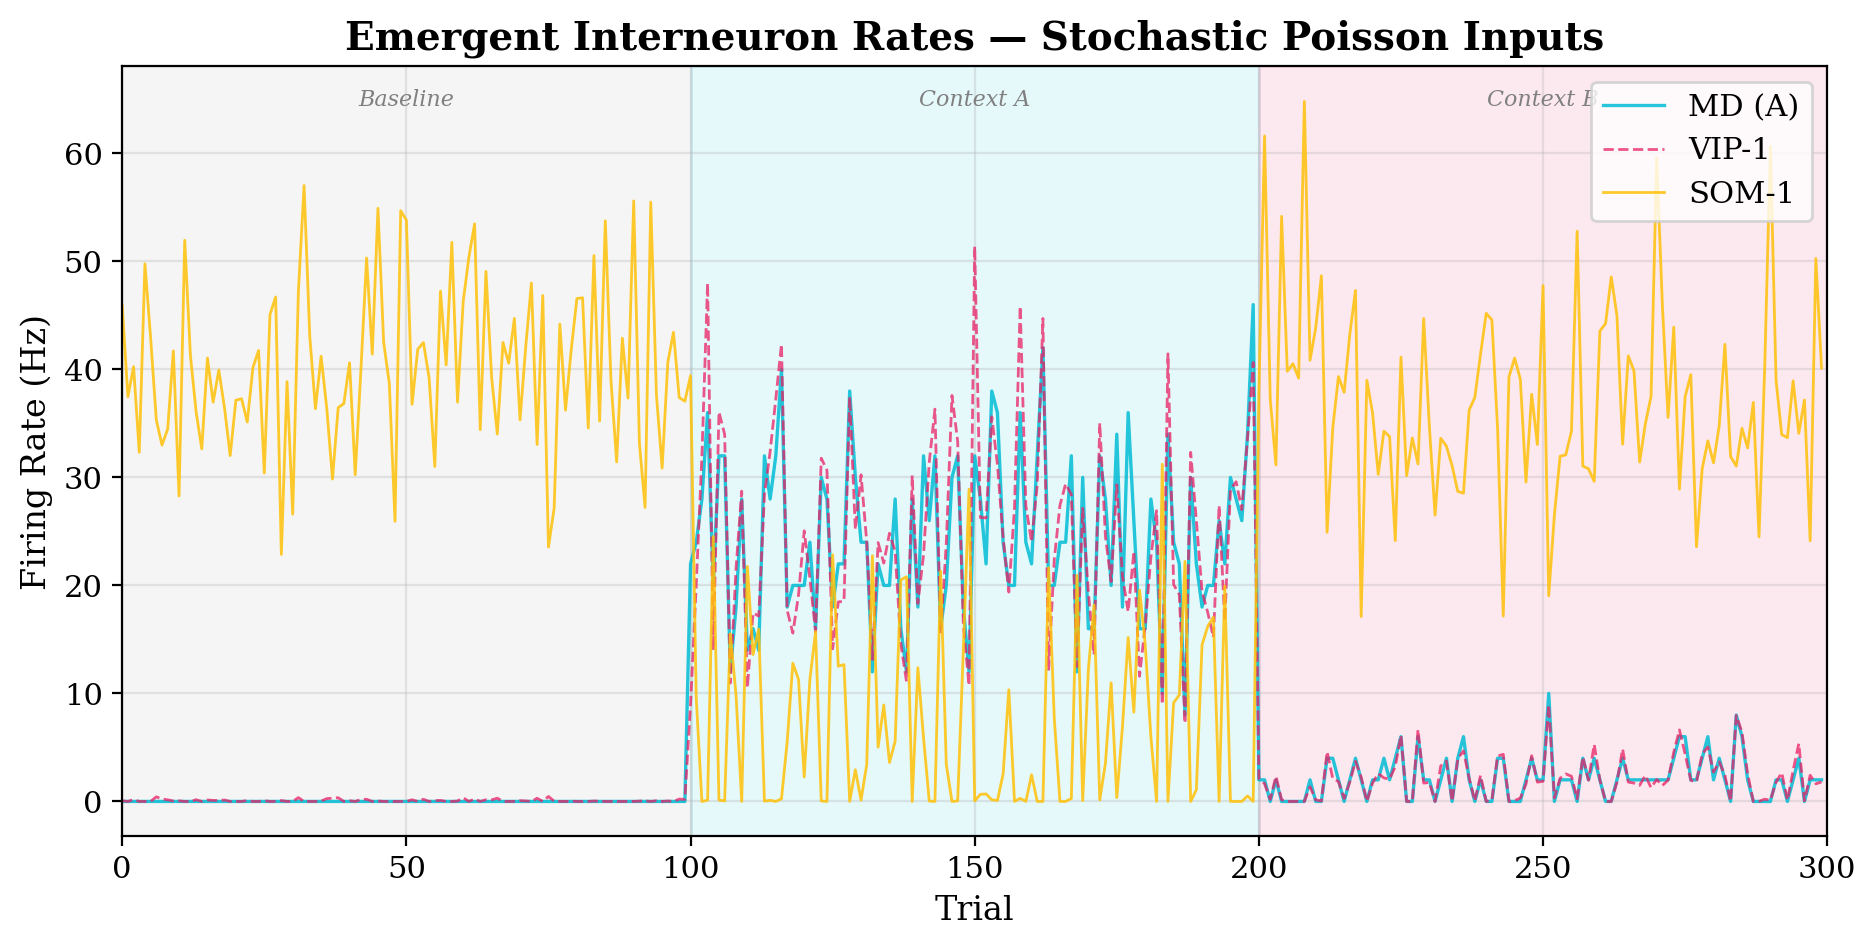
\includegraphics[width=\textwidth]{figures/mechanistic/fig_emergent_rates.png}
        \caption{Stochastic interneuron firing rates}
    \end{subfigure}
    \hfill
    \begin{subfigure}[b]{0.48\textwidth}
        \centering
        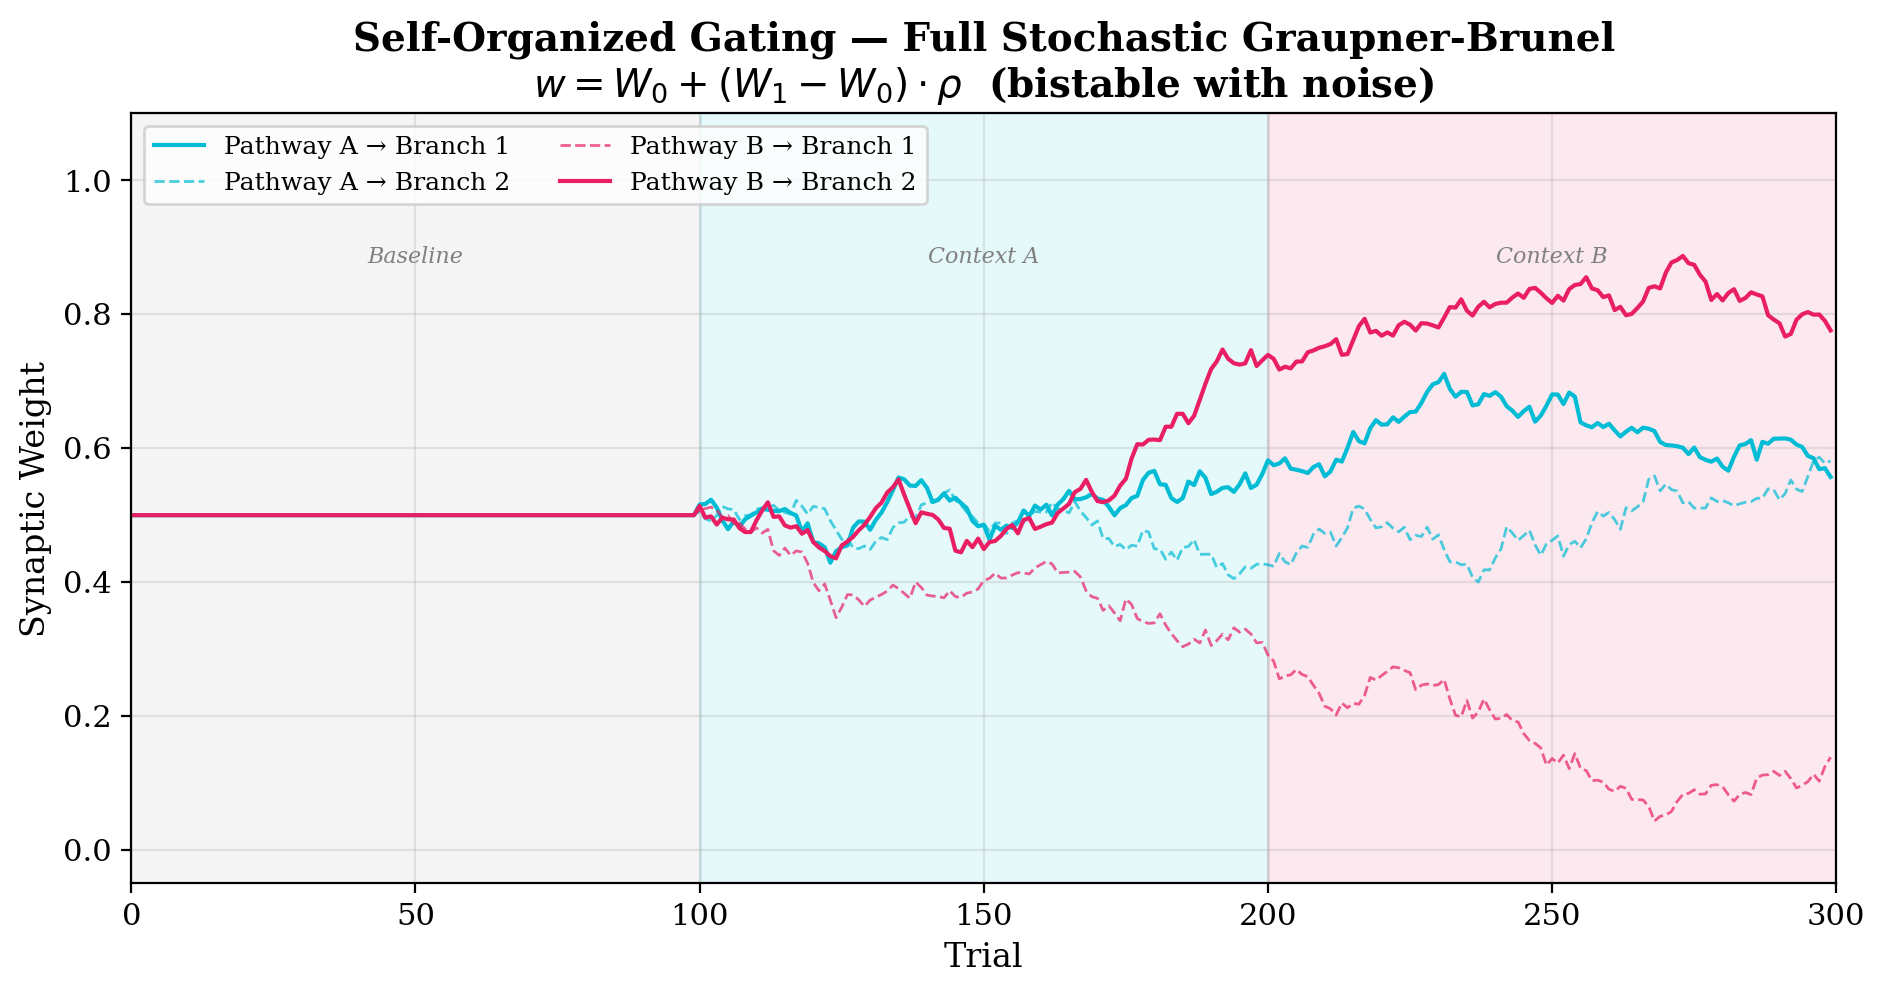
\includegraphics[width=\textwidth]{figures/mechanistic/fig_self_organized_branching.png}
        \caption{Weight trajectories under emergent inhibition}
    \end{subfigure}
    \caption{Output from the emergent mechanistic model. Panel (a) shows the intended
    circuit behaviour and is verified. Panel (b) does \textbf{not} currently show
    branch-specific learning --- see the box below.}
    \label{fig:mechanistic_output}
\end{figure}

\begin{gapbox}{Plasticity is currently inert in both figure models}
Instrumenting every Graupner-Brunel update shows that \emph{all} of them fall through
to the calcium-inactive branch: 400/400 in \texttt{main\_gating\_figures.make\_figure4}
and 800/800 in \texttt{emergent\_gating\_mechanistic\_model}. Peak calcium reaches
$\approx 0.80$ against $\theta_D = 1.0$, so neither threshold is ever crossed.

Consequently Figure \ref{fig:phenom_learning} and Figure
\ref{fig:mechanistic_output}(b) show an \textbf{unbiased random walk} driven only by
$\sigma_\rho$, not learning; and $\eta_\rho$, $\bar{\rho}$, $\gamma_D$, $\gamma_P$, the
Mg$^{2+}$ block and the \texttt{CV\_CA} vesicle noise have no effect on the output.
The random walk also currently favours the \emph{wrong} branch (at the end of Context
A: pathway~A~$\rightarrow$~branch~1 $= 0.563$ versus
pathway~A~$\rightarrow$~branch~2 $= 0.739$).

\textbf{Root cause.} The \texttt{dend\_IO} transfer function is inverted in the regime
these models occupy. Since $\text{spread} = q_1 e^{\,\text{inh}/q_2}$ reaches
$\approx 2000$ nS at $35$ nS of inhibition while the models generate only $0.7$--$3.8$
nS of excitation, the sigmoid never leaves its floor --- and that floor \emph{rises}
with inhibition. A branch under $32.4$ nS of inhibition reports $-43.6$ mV while a
branch under $2.2$ nS reports $-68.8$ mV, giving a \emph{larger} Mg$^{2+}$ unblock on
the branch that should be shut. Four separate copies of this function exist. Fixing it
requires a decision about the dendritic operating point and will change every figure,
so it is deliberately left unapplied here.
\end{gapbox}

\section{Experimental Protocol: The 3-Epoch Paradigm}
To test the models' ability to learn and switch contexts, we designed a continuous
\textbf{300-trial} simulation ($500$ ms per trial) divided into three equal epochs.
\textbf{This protocol is implemented in Model C only.}

\begin{table}[H]
    \centering
    \small
    \begin{tabular}{@{}llp{2.8cm}p{3.6cm}p{3.4cm}@{}}
    \toprule
    \textbf{Epoch} & \textbf{Trials} & \textbf{MD Drive} & \textbf{Circuit State} & \textbf{Intended Outcome} \\ \midrule
    \textbf{Baseline} & 0--99 & 0 Hz both channels & VIP silent, SOM $= 40$ Hz, both branches inhibited at $35$ nS & No learning; weights stable \\ \addlinespace
    \textbf{Context A} & 100--199 & 25 Hz to VIP-1, \textbf{2 Hz} to VIP-2 & VIP-1 suppresses SOM-1 to $2.5$ Hz; branch 1 at $2.2$ nS, branch 2 at $32.4$ nS & Pathway A potentiates on branch 1 \\ \addlinespace
    \textbf{Context B} & 200--299 & \textbf{2 Hz} to VIP-1, 25 Hz to VIP-2 & Mirror image; branch 2 disinhibited & Pathway B potentiates on branch 2, branch 1 retained \\ \bottomrule
    \end{tabular}
    \caption{The 3-epoch simulation protocol as implemented in Model C. Note the
    \textbf{2 Hz background floor} on the non-preferred channel: it is not silent.
    Earlier versions of this table omitted it, which matters for interpreting the
    selectivity indices in Section \ref{sec:gs}.}
    \label{tab:protocol}
\end{table}

\begin{gapbox}{The baseline epoch does not currently test the gate}
Both figure models skip the plasticity update entirely when the pathway rate is zero
(\texttt{continue}), so during trials 0--99 the weights hold at $\rho = 0.5$ by
short-circuit rather than because inhibition blocks learning. The two models also use
\emph{different} skip conditions --- Model B tests \texttt{r\_pre} alone, Model C tests
\texttt{r\_pre} \emph{and} \texttt{g\_exc} --- which is why Model B's Figure 4 shows
two moving traces and Model C's shows four.
\end{gapbox}

\begin{gapbox}{This protocol is absent from the Brian 2 model}
Model A implements no equivalent. \texttt{demo\_v2\_zhang2025.py} switches
\emph{global} MD drive from $5$ Hz to $40$ Hz over $2 + 2$ seconds and labels those
levels ``Context A'' and ``Context B''; there are no separate VIP-1/VIP-2 channels, no
branch-selective targeting and no baseline epoch.
\texttt{sweep\_phase\_diagram.py} runs a single fixed context at $40$ Hz. Porting the
3-epoch paradigm to Model A remains outstanding work.
\end{gapbox}

\section{Quantifying Circuit Behaviour: Gating Selectivity}
\label{sec:gs}
To confirm that the interneurons perform their designated roles in Model C, we measure
the \textbf{Gating Selectivity (GS) index} --- how strongly a cell prefers its target
context over the opposing one:
\begin{equation}
    GS = \frac{r_{\text{preferred}} - r_{\text{non-preferred}}}
              {r_{\text{preferred}} + r_{\text{non-preferred}}}
\end{equation}

The measured values reproduce exactly from seed 42:
\begin{itemize}
    \item \textbf{VIP $GS = 0.86$:} highly selective --- fires strongly in its target
      context.
    \item \textbf{SOM $GS = -0.66$:} strongly anti-selective --- suppressed in the
      target context, which is the signature of successful disinhibition.
    \item \textbf{PV $GS = 0.01$:} non-selective --- responds equally to both contexts,
      consistent with a global gain-control role.
\end{itemize}

\paragraph{A correction to the stated cause.}
Earlier versions of this document attributed the departure from a ``suspiciously
perfect'' $GS = 1.0$ to Poisson noise. That is not the dominant factor. The
$2$ Hz background floor of Table \ref{tab:protocol} alone predicts
\begin{equation}
    GS_{\text{VIP}} = \frac{25 - 2}{25 + 2} = 0.85,
\end{equation}
which accounts for essentially the entire gap from unity. For SOM, the additional
departure from the deterministic prediction of $-0.87$ to the measured $-0.66$ comes
mainly from rectification: $\max(0, 40 - 1.5\,r_{\text{VIP}})$ is a biased estimator
when $r_{\text{VIP}}$ is itself noisy and the argument sits near zero. Poisson noise
contributes, but the protocol design and the rectifier dominate. The values remain
realistic; the mechanism behind them is simply not the one previously claimed.

\begin{figure}[H]
    \centering
    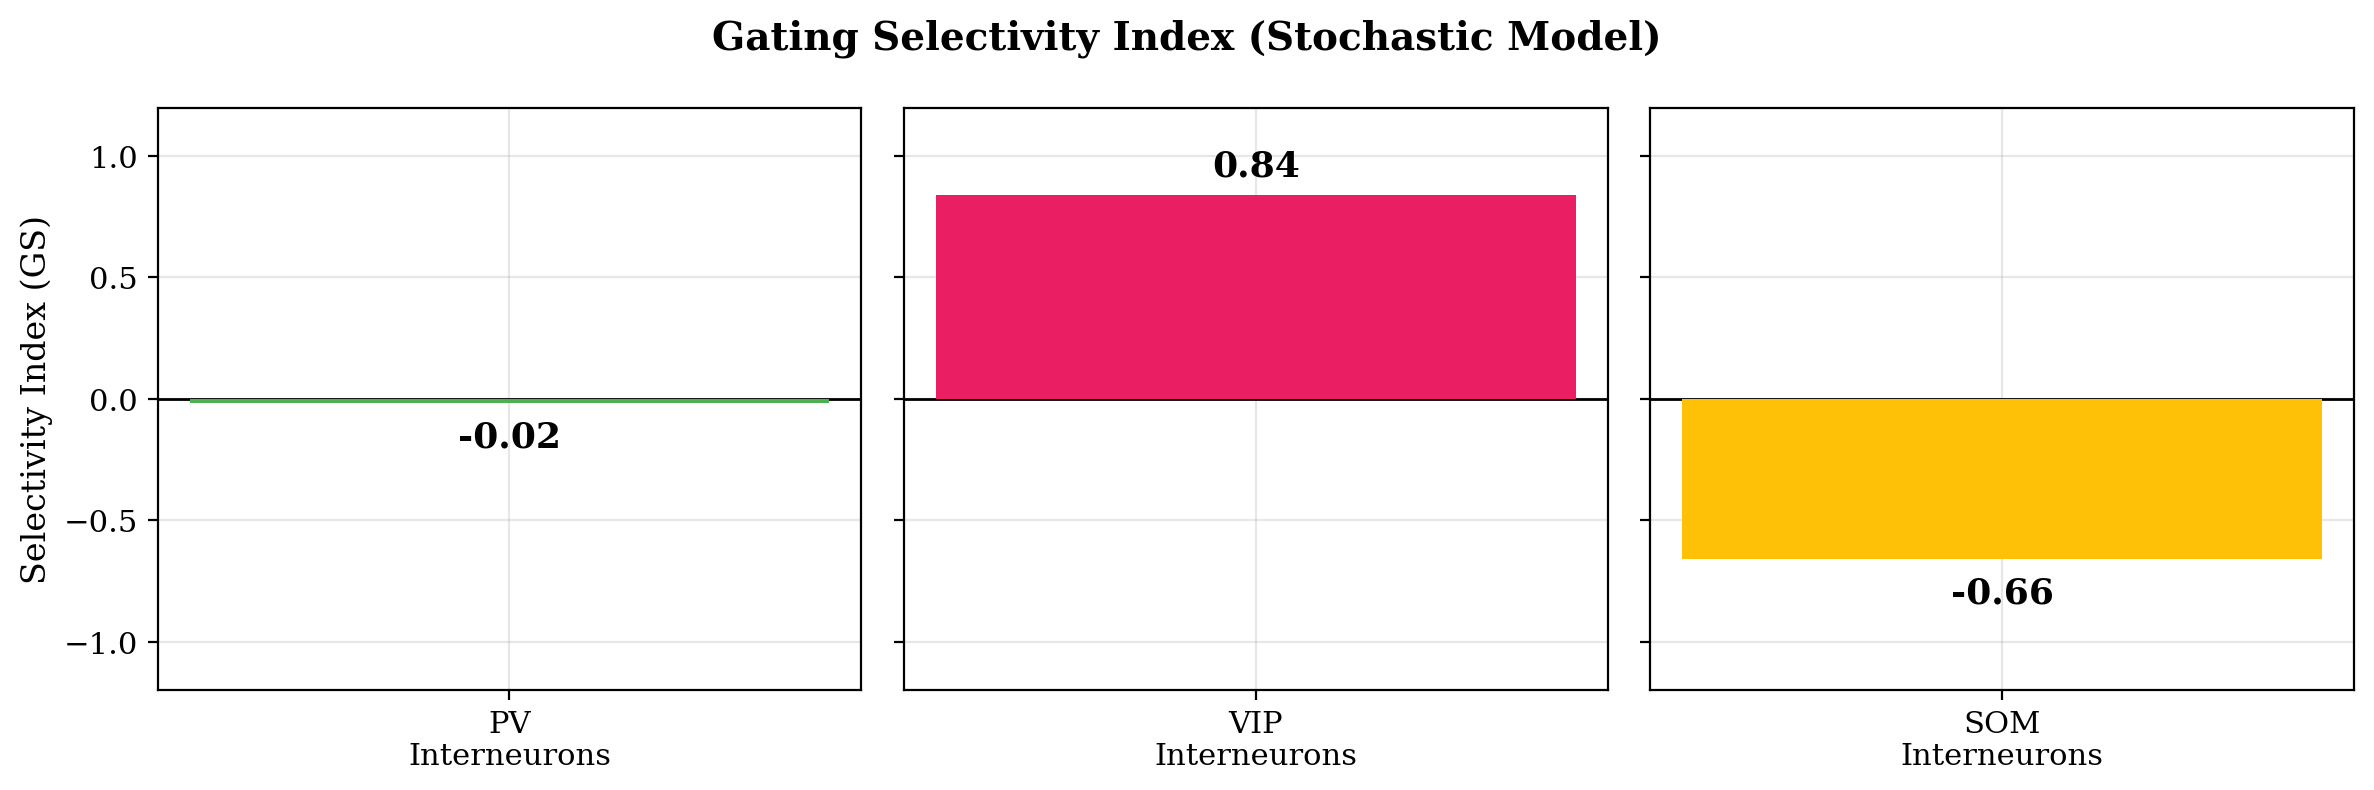
\includegraphics[width=0.75\textwidth]{figures/mechanistic/fig_gating_selectivity.png}
    \caption{Gating Selectivity indices for the three interneuron classes.}
    \label{fig:gs_scores}
\end{figure}

\section{Verification Status}
\label{sec:verification}
Everything below was established by executing the code, not by reading it. The
automated suite (\texttt{experiments/validate\_model.py}, $\approx$904 s) currently
reports \textbf{5/6 passing}.

\begin{okbox}{Verified working}
\begin{itemize}
    \item \textbf{MD $\rightarrow$ VIP $\rightarrow$ SOM disinhibition (Model A).}
      The gate opens and closes as specified: SOM fires at $36.5$ Hz when MD is at
      $5$ Hz (gate closed) and is fully silenced at $20$ Hz MD drive (gate open);
      VIP reaches $35.2$ Hz at $25$ Hz MD drive. This is the core circuit motif and it
      works.
    \item \textbf{Calcium kinetics (Model A).} Exact to numerical precision: a single
      pre-spike gives a peak of $1.000$ against $C_{\text{pre}} = 1.0$, decaying to
      $0.368$ after one $\tau_{\text{Ca}}$ ($1/e = 0.3679$).
    \item \textbf{Rate-coded plasticity direction (Model A).} $100$ Hz input drives
      $\rho: 0.50 \rightarrow 0.738$ (LTP); $40$ Hz drives
      $\rho: 0.50 \rightarrow 0.069$ (LTD). The bistable machinery functions.
    \item \textbf{Numerical stability.} No NaN or Inf across a $10$ s full-circuit
      simulation; weights remain within $[0, 3]$.
    \item \textbf{Reproducibility.} Seeded runs are bit-reproducible; the GS values of
      Section \ref{sec:gs} regenerate exactly.
    \item \textbf{The parameters of Section \ref{sec:poisson}} match
      \texttt{parameters.py} exactly, and the $40$ Hz SOM baseline is empirically
      confirmed.
\end{itemize}
\end{okbox}

\begin{gapbox}{Blocking issue: dendritic inhibition does not gate plasticity in Model A}
This is the single most consequential gap. The synaptic calcium equation is
\begin{equation}
    \frac{dc}{dt} = -\frac{c}{\tau_{\text{Ca,NMDA}}},
    \qquad c \mathrel{+}= C_{\text{pre}} \text{ on each presynaptic spike,}
\end{equation}
with \textbf{no} postsynaptic voltage term, \textbf{no} NMDA Mg$^{2+}$ block and
\textbf{no} coincidence detection. The \texttt{on\_post\_plasticity} rule
($c \mathrel{+}= C_{\text{post,eff}}$) is defined in \texttt{equations.py} and imported
by \texttt{MultiCompartmentalModel.py}, but is \emph{never attached to any}
\texttt{Synapses} \emph{object}; \texttt{C\_post\_eff} is not even defined in
\texttt{parameters.py}.

Synaptic calcium is therefore a function of the presynaptic Poisson train alone. Two
branches receiving the same afferents evolve identically no matter how differently they
are inhibited, so pathway-specific gating cannot occur by construction. This is the
direct cause of the failing test:
\begin{center}
\texttt{TEST 3: Branch-Specific Gating}\\
\texttt{Branch 0 (inhibited): 1.484 \quad Branch 1 (disinhibited): 1.474}\\
\texttt{Ratio (free / inhibited): 0.99 -> FAIL}
\end{center}
The ratio falling \emph{below} unity is the expected signature of two statistically
identical processes with independent noise.
\end{gapbox}

\begin{gapbox}{MD $\rightarrow$ PV somatic gain control is non-functional}
$g_{\text{AMPA,PV}} = 0.12$ nS is too weak to bring PV to threshold across the
operating range. Measured PV population rates: $0.0$ Hz at both $5$ Hz and $25$ Hz MD
drive, $2.9$ Hz at $40$ Hz, then $184.7$ Hz at $100$ Hz --- essentially no usable
dynamic range. Tests 4 and 5 independently report PV $= 0.0$ Hz, and Test 4 shows the
pyramidal cell firing at $50.6$ Hz with no inhibitory opposition. The E/I balance arm
of the Zhang (2025) hypothesis is therefore not yet exercised by the model.
\end{gapbox}

\begin{gapbox}{Other specified features not yet implemented}
\begin{itemize}
    \item \textbf{No pathology classification in the phase diagram.}
      \texttt{sweep\_phase\_diagram.py} emits four raw heatmaps (PV, SOM and Pyr rates,
      and $\Delta W$) and marks a single point labelled ``Healthy Baseline'' at the
      default weights. There is, however, no \emph{pathological} regime, no boundary
      between regimes and no classification logic --- so the intended ``healthy
      flexibility versus pathology'' mapping currently amounts to one annotated point.
      Because $\rho$ cannot depend on the swept MD$\rightarrow$PV /
      MD$\rightarrow$VIP weights, the $\Delta W$ panel additionally carries no
      information.
    \item \textbf{\texttt{print\_network\_summary.py} does not inspect a live network.}
      It constructs no Brian 2 objects; the report body is string literals, and seven
      of its ten stated facts are wrong (30 branches versus 2; 10 PV/SOM/VIP versus 20
      each; 20 MD cells versus 50; $p = 0.50$ for VIP$\rightarrow$SOM and
      PV$\rightarrow$Soma versus $0.6$). Only the imported equation block is genuine.
    \item \textbf{Figure 1 has no LTP arm.} $C_{\text{NMDA}} + C_{\text{bAP}} = 1.328$
      lies below $\theta_P = 2.78$, so a single pre-post pair cannot reach the
      potentiation threshold at any $\Delta t$ and the plotted STDP curve is LTD-only.
      The constants appear to mix two different Graupner-Brunel fits
      ($\tau_\rho$ and $\sigma$ from one; $C$, $\theta$ and $\gamma$ from another).
      \textbf{This should be resolved against the source paper before any further
      parameter tuning}, since every recalibration depends on which set is
      authoritative.
    \item \textbf{Figure 3's NMDA calcium is identically zero.} The driving-force term
      $\max(v_{\text{dend}} + 10, 0)$ is always $0$ because $v_{\text{dend}}$ never
      exceeds $-10$ mV in that figure's range, so all of its calcium comes from the
      bAP term and the Mg$^{2+}$-block computation is inert. No curve crosses
      $\theta_P$, so the plotted ``LTP zone'' band is never entered.
    \item \textbf{$\rho$ noise is not calcium-gated in Model A}, so a silent synapse
      drifts away from its initial state; and only $w$ is clipped to $[0,1]$, not
      $\rho$ itself, so $\rho$ can leave the double well.
    \item \textbf{$w_1$ is inconsistent across models} --- $3.0$ in
      \texttt{parameters.py} and Model B, $1.0$ in Model C --- so the two Figure-4-style
      weight axes are not directly comparable despite carrying the same caption.
\end{itemize}
\end{gapbox}

\section{Reproducing the Figures}
All commands assume the project's conda interpreter; there is no \texttt{python} on
\texttt{PATH}, and the system \texttt{python3} has no Brian 2.

\begin{table}[H]
    \centering
    \small
    \begin{tabular}{@{}llll@{}}
    \toprule
    \textbf{Figure} & \textbf{Script} & \textbf{Runtime} & \textbf{Output} \\ \midrule
    \ref{fig:architecture}
      & \texttt{experiments/generate\_network\_synapse\_figure.py} & 3 s
      & \texttt{figures/} \\
    1--4, \ref{fig:phenom_learning}
      & \texttt{main\_gating\_figures.py} & 3 s
      & \texttt{figures/phenomenological/} \\
    \ref{fig:mechanistic_output}, \ref{fig:gs_scores}
      & \texttt{emergent\_gating\_mechanistic\_model.py} & 4 s
      & \texttt{figures/mechanistic/} \\
    validation
      & \texttt{experiments/validate\_model.py} & 904 s
      & \texttt{figures/validation/} \\
    phase diagram
      & \texttt{experiments/sweep\_phase\_diagram.py} & 171 s
      & \texttt{figures/phase\_diagram.png} \\
    context switch
      & \texttt{experiments/demo\_v2\_zhang2025.py} & minutes
      & \texttt{figures/} \\ \bottomrule
    \end{tabular}
    \caption{Verified commands and measured runtimes. See \texttt{README.md} for the
    interpreter path and environment notes.}
\end{table}

\section*{References}
\begin{itemize}
    \item \textbf{Yang et al.\ 2016:} ``A dendritic disinhibitory circuit mechanism for
      pathway-specific gating'', \textit{Nature Neuroscience}.
    \item \textbf{Graupner \& Brunel 2012:} ``Calcium-based plasticity model explains
      sensitivity of synaptic changes to spike pattern, rate, and dendritic location'',
      \textit{PNAS}.
    \item \textbf{Zhang 2025:} MD thalamocortical drive, E/I imbalance, and context
      learning.
\end{itemize}

\end{document}
